\chapter{Conclusion}
En somme, le projet portant sur la simulation d'un accélérateurs de particules fut un succès. Le cahier des charges du client au niveau de la dynamique des simulateurs a été respecté. L'outil de dimensionnement livré permet de faire varier les paramètres dans les simulations et de les lancer. Les simulations sont représentatives du comportement observé au CERN, si l'on se réfère aux courbes qui ont été fournies par le client. Ils permettent de compléter le cahier des charges. La section portant sur le simulateur temps réel n'est pas complète suivant des retards dans la livraison et l'installation des simulateurs. Cependant, il a été possible de documenter l'installation et l'utilisation, ce qui pour le client était le plus important. Pour ce qui est des avancées possible dans le projet, il est évident que l'intégration du convertisseur \og Trim \fg{} présenté à la figure \ref{conv_CERN} doit être réalisée. Ce convertisseur permet l'emploi d'inductances de couplage de plus grande impédance et donc une ondulation moins élevée du courant de sortie. De plus, les contrôles utilisés dans le projet sont des contrôles classiques fait de régulateurs PID. Les régulateurs employés au CERN sont des régulateurs RST qui sont réalisés exclusivement dans un modèle discret. Ils permettent une souplesse de réglage supérieure ainsi qu'une optimisation des paramètres des réglages.


\begin{figure}[htb]
\centering
\makebox[\textwidth][c]{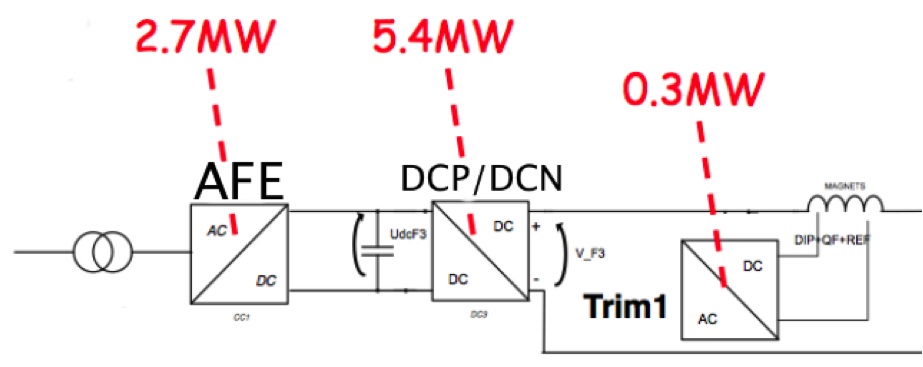
\includegraphics[scale=0.75]{fig/convertisseur_CERN.png}}
\caption{Schéma bloc de la chaîne de convertisseurs alimentant les électroaimants du CERN}
\label{conv_CERN}
\end{figure}
